\title{Unsupervised, parts based object detection}
\author{
        Alex Kreimer \\
                Department of Computer Science\\
        Technion
}
\date{\today}

\documentclass[12pt]{article}

\usepackage{subfig}
\usepackage[english]{babel}
\usepackage{graphicx}
\usepackage{amssymb,amsmath}
\usepackage{caption}

\DeclareMathOperator*{\argmin}{arg\,min}


\begin{document}
\maketitle

\begin{abstract}

This project is submitted as part of the requirements for the Computer Vision seminar under the supervision of prof. Micha Lindenbaum. \\ We've built an algorithm that is capable of learning object appearance in a parts-based fashion and apply this knowledge to detect objects in novel images.  The algorithm was tested using car image database that was built during the project.
\\ The results show that the algorithm chose some number of relevant features (e.g. various car parts) along with some irrelevant features.  The ROC of the classifier suggest that for robust object detection the algorithm should be improved

\end{abstract}

\section{Intro}
The goal of this project is to implement an unsupervised parts based object detection algorithm.  The training algorithm is presented in section~\ref{training}.
\paragraph{Features} We treat square image patches as features.  Size of a patch is a parameter to the algorithm.  The results that are presented in this report are produced with patch size of $[41,41]$
\paragraph{Distance from feature to image} The distance between feature and image is defined as a minimum of distances between feature and any possible square patch in the image.  Note that the patch similarity measure function is a parameter to the algorithm.  To produce the results presented here we've used the normalized cross correlation.


\section{Training Algorithm}\label{training}

\begin{enumerate}
\item Designate a number of positive images as 'model' images.  Choose candidate features from model images over a sparse grid.  See Figure~\ref{fig:sub2} for grid example.
\item For each feature, calculate its distance to all training images (both positive and negative).
\item For each feature, calculate the distance threshold that minimizes its training set classification error . See subsection~\ref{calc_thresh} for details.
\item Select the most discriminative features from the set of all candidate features (the number of features is a parameter to the algorithm). See~\ref{feat_sel} for details
\item For each training image calculate a descriptor as explained in subsection~\ref{descriptors} and train SVM.
\end{enumerate}

\begin{figure} \centering
	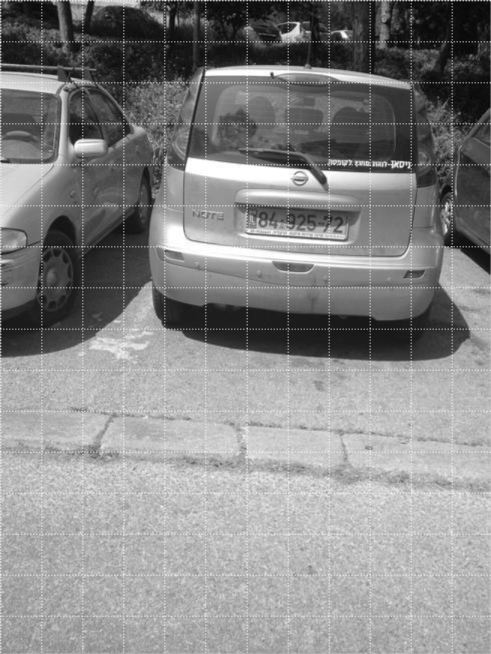
\includegraphics[width=.4\linewidth]{model_feats.png}
	\caption{Model features over a grid}
	\label{fig:sub2}
\end{figure}

\subsection{Distance thresholds}\label{calc_thresh}
We think of each feature as a simple classifier.  If its distance to image is less than the threshold, the classification outcome is positive and negative otherwise. We accumulate feature distances to positive/negative images in a pair of histograms.  Going over bin boundaries we find a threshold that minimizes the number of mis-classifications for our training set.

\subsection{Feature selection}\label{feat_sel}
Since usually there's a large number of candidate features, we need to choose some small subset of them.  One way to do this is a simple greedy algorithm that selects a feature(s) that had the smallest number of mis-classifications while calculating the thresholds.  One disadvantage of such approach is that similar features may be chosen.  We apply a variation of boosting procedure, which begins with uniform weights for all training set images.  At each iteration we double the weight of the mis-classified image, and half the weight of correctly classified images.  When choosing the feature, its correct and incorrect classifications are weighted with their corresponding weights.
\subsection{Image descriptors}\label{descriptors}
For each image we build a descriptor vector.  The length of a vector is a number of features chosen in subsection~\ref{feat_sel}.  Each coordinate correspond to a single feature and is 1 if the distance from the image to this feature is less than this features' threshold and 0 otherwise.

\section{Detection Algorithm}
For a novel image we calculate its descriptor exactly as stated in subsection~\ref{descriptors} and test against the trained SVM.

\section{Training database}\label{db}

\begin{figure} \centering
	\subfloat[][Image\#1]{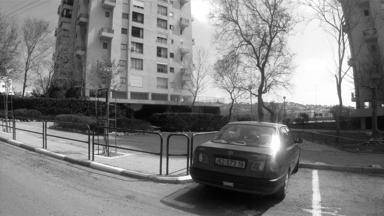
\includegraphics[width=.4\linewidth]{sample1.jpg}\label{<figure1>}}
 	\subfloat[][Image\#2]{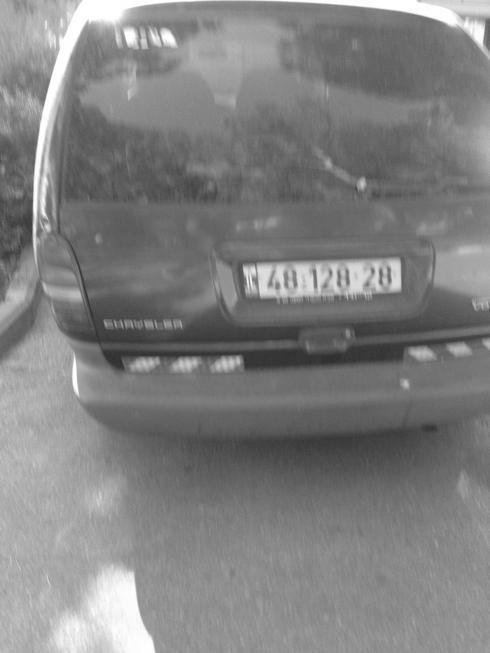
\includegraphics[width=.4\linewidth]{sample2.jpg}\label{<figure2>}}
	\caption{Car images in the database}
	\label{fig:sub1}
\end{figure}

The project required training/test database.  A collection of images was made that contained cars.  The images were made using a hand held mobile device camera.  Most of the images were made during the morning/noon hours which means lots of sun and some shades. Please see Figure ~\ref{fig:sub1} for  an example of a random images from the database.

\section{Various distance measures}

During the testing we've experimented with different distance measures except ncc, which also include SAD, SSD.  We didn't see a significant performance gain using any one of the metrics.

\section{Results}

\paragraph{Selected features.}  One of the goals of the algorithm was to choose the most discriminative features, that separated well the images that have cars against the images that don't.  The Figure~\ref{sub3} has patches that were selected by the algorithm.  One may see that part of the images are indeed the parts of the car, while significant part is just 'noise'.  I think that the reason for this is insufficient training data.
\paragraph{ROC} To train and assess the performance of the SVM we used n-fold (n=10) cross-validation technique. See Figure~\ref{ROC} for the ROC.  Cross-validation splits the data into the training set and the test set (usually 10\% of the data is used for testing).  The SVM is trained using the training set and tested using the test set.  The process is repeated n times and the results are averaged to obtain the attached graph.  One may see that the algorithm will detect about 85\% of cars while producing 10\% false positive results.

\begin{figure} \centering
	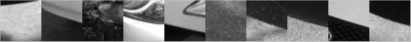
\includegraphics[width=.4\linewidth]{good_features.png}
	\caption{The features selected by the algorithm}
	\label{fig:sub3}
\end{figure}

\begin{figure} \centering
	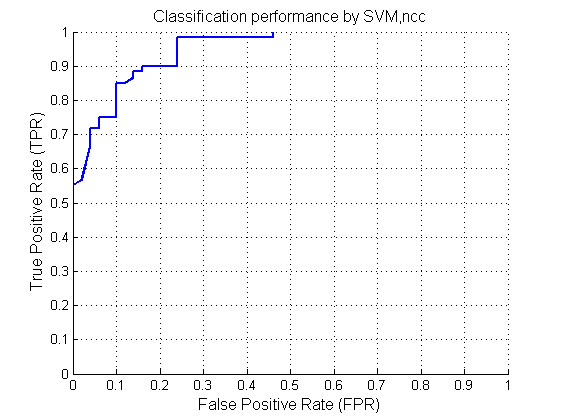
\includegraphics{roc.png}
	\caption{ROC}
	\label{fig:sub4}
\end{figure}

\section{Conclusions}

While the method performs at a level satisfactory for a small project in may be greatly improved in many respects.  To name a few:
\begin{enumerate}
\item Better dataset should be prepared
\item More appropriate features should be used (allowing at least some tolerance to variability of views and lighting)
\end{enumerate}
\end{document}
This is never printed